\documentclass[12pt]{article}

\usepackage[utf8]{inputenc}
\usepackage[spanish]{babel}
\usepackage{amssymb, amsmath, geometry, graphicx}

\setlength{\parindent}{0cm}
\geometry{letterpaper, margin=2.54cm}
\decimalpoint
\pagestyle{plain}

\title{
	Geometría Analítica Vectorial y Funciones Vectoriales \\
	\vspace{0.4cm}
	\Large Graficación de Curvas Planas en Coordenadas Polares
}
\date{21 de junio de 2026}
\author{Rosendo Camal}

\begin{document}

% Portada
\maketitle

% Actividad 1
\section*{Actividad 1}
\textbf{Instrucciones:} Construir la tabla y graficar $r = 4$.
\newline

\textbf{Respuesta:} Considerando el par ordenado $(x, y)$ equivalente a $\left( r\cdot\cos\theta, r\cdot\sin\theta \right)$:

\begin{center}
	\begin{tabular}{| c | c | c | c | c |}
		\hline
		$\theta$ & $r$ & $(r, \theta)$ & $(x, y)$ \\ \hline
		0 & 4 & $\left(4, 0\right)$ & $(4, 0)$\\
		$\frac{\pi}{4}$ & 4 & $\left(4, \frac{\pi}{4}\right)$ & $(2\sqrt{2}, 2\sqrt{2})$ \\
		$\frac{\pi}{2}$ & 4 & $\left(4, \frac{\pi}{2}\right)$ & $(0, 4)$ \\
		$\frac{3\pi}{4}$ & 4 & $\left(4,\frac{3\pi}{4}\right)$ & $(-\sqrt{2}, 2\sqrt{2})$ \\
		$\pi$ & 4 & $\left(4, \pi\right)$ & $(-4, 0)$ \\
		$\frac{5\pi}{4}$ & 4 & $\left(4, \frac{5\pi}{4}\right)$ & $(-2\sqrt{2}, -2\sqrt{2})$ \\
		$\frac{3\pi}{2}$ & 4 & $\left(4, \frac{3\pi}{2}\right)$ & $(0, -4)$ \\
		$\frac{7\pi}{4}$ & 4 & $\left(4, \frac{7\pi}{4}\right)$ & $(2\sqrt{2}, -2\sqrt{2})$ \\
		$2\pi$ & 4 & $\left(4, 2\pi\right)$ & $(4, 0)$ \\
		\hline
	\end{tabular}
\end{center}

\begin{figure}[htb]
	\centering
	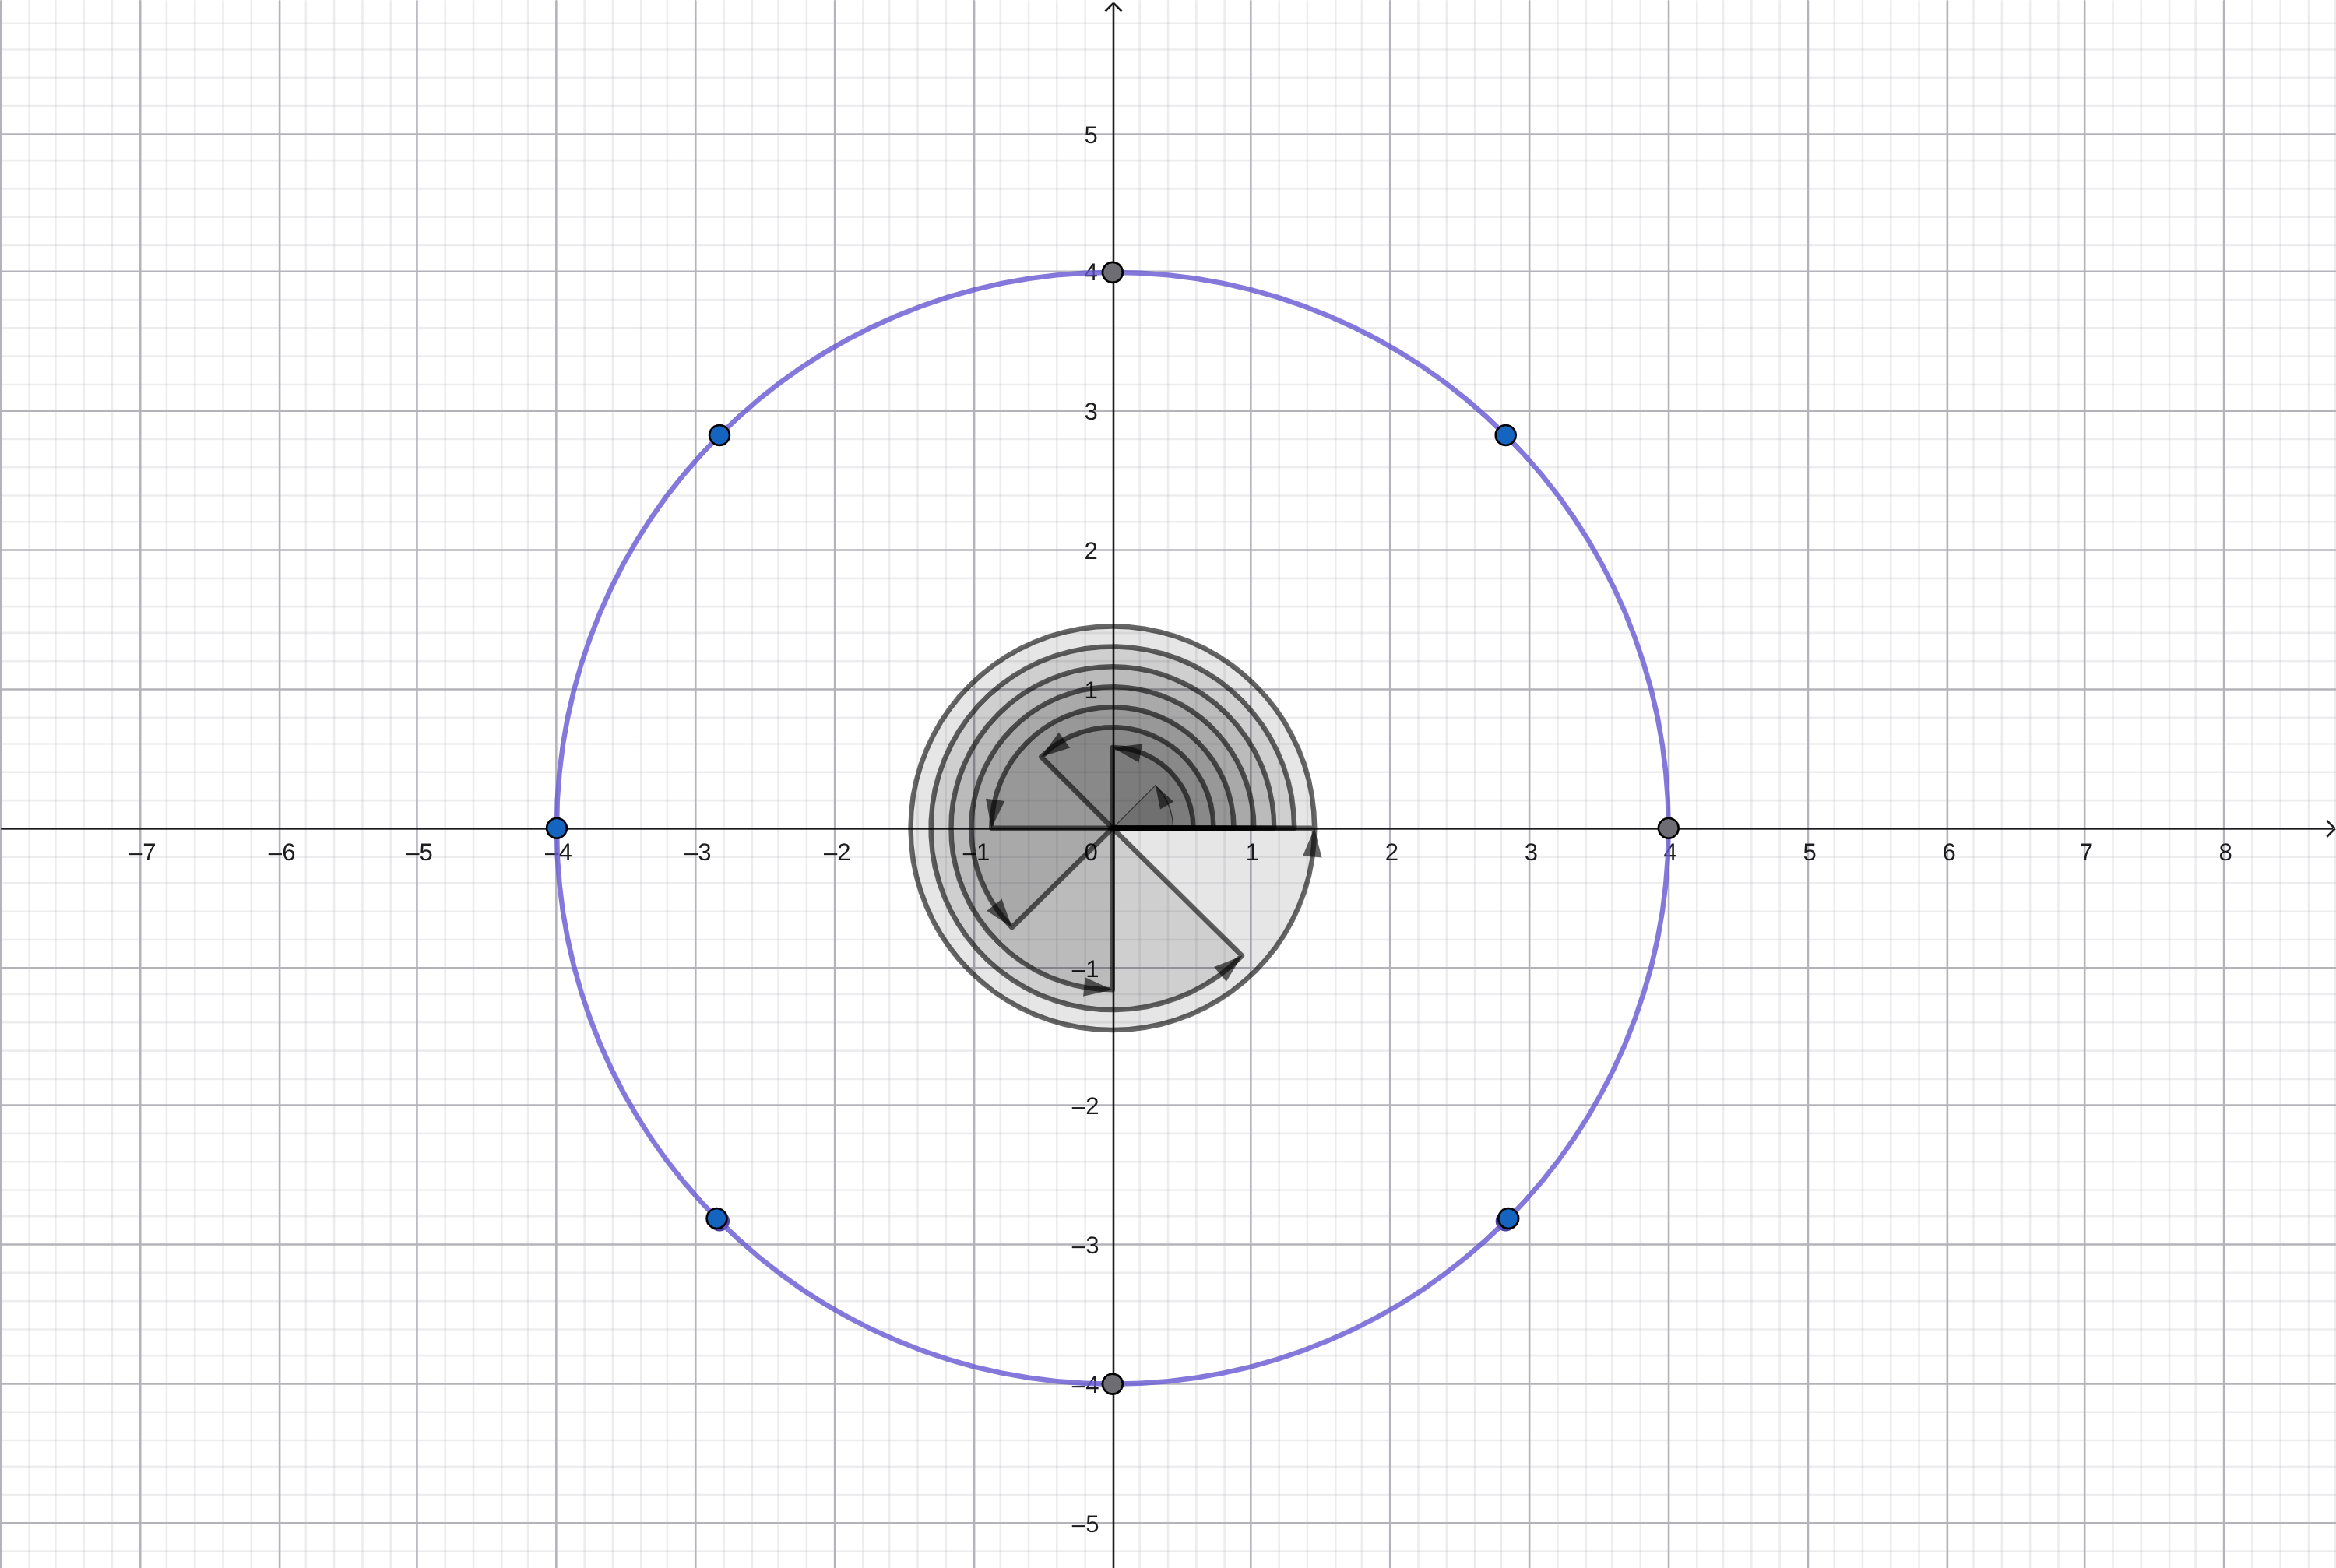
\includegraphics[width=0.6\linewidth]{./geogebra-export1.png}
\end{figure}

% Actividad 2
\section*{Actividad 2}
\textbf{Instrucciones:} Construir la tabla y graficar $r = 2\cdot\cos\theta$ para $0^\circ, 30^\circ, 60^\circ, 90^\circ, 120^\circ, 150^\circ, 180^\circ$.
\newline

\textbf{Respuesta:} Considerando a $(x, y)$ equivalente a $\left(r\cdot\cos\theta, r\cdot\sin\theta\right)$:

\begin{center}
	\begin{tabular}{| c | c | c | c |}
		\hline
		$\theta$ & $r$ & $(r, \theta)$ & $(x, y)$ \\ \hline
		$0^\circ$ & 2 & $(2, 0^\circ)$ & $(2, 0)$ \\
		$30^\circ$ & $\sqrt{3}$ & $(\sqrt{3}, 30^\circ)$ & $(\frac{3}{2}, \frac{\sqrt{3}}{2})$ \\
		$60^\circ$ & 1 & $(1, 60^\circ)$ & $(\frac{1}{2}, \frac{\sqrt{3}}{2})$ \\
		$90^\circ$ & 0 & $(0, 90^\circ)$ & $(0, 0)$ \\
		$120^\circ$ & $-1$ & $(-1, 120^\circ)$ & $(\frac{1}{2}, -\frac{\sqrt{3}}{2})$ \\
		$150^\circ$ & $-\sqrt{3}$ & $(-\sqrt{3}, 150^\circ)$ & $(\frac{3}{2}, -\frac{\sqrt{3}}{2})$ \\
		$180^\circ$ & $-2$ & $(-2, 180^\circ)$ & $(2, 0)$ \\
		\hline
	\end{tabular}
\end{center}

\begin{figure}[htb]
	\centering
	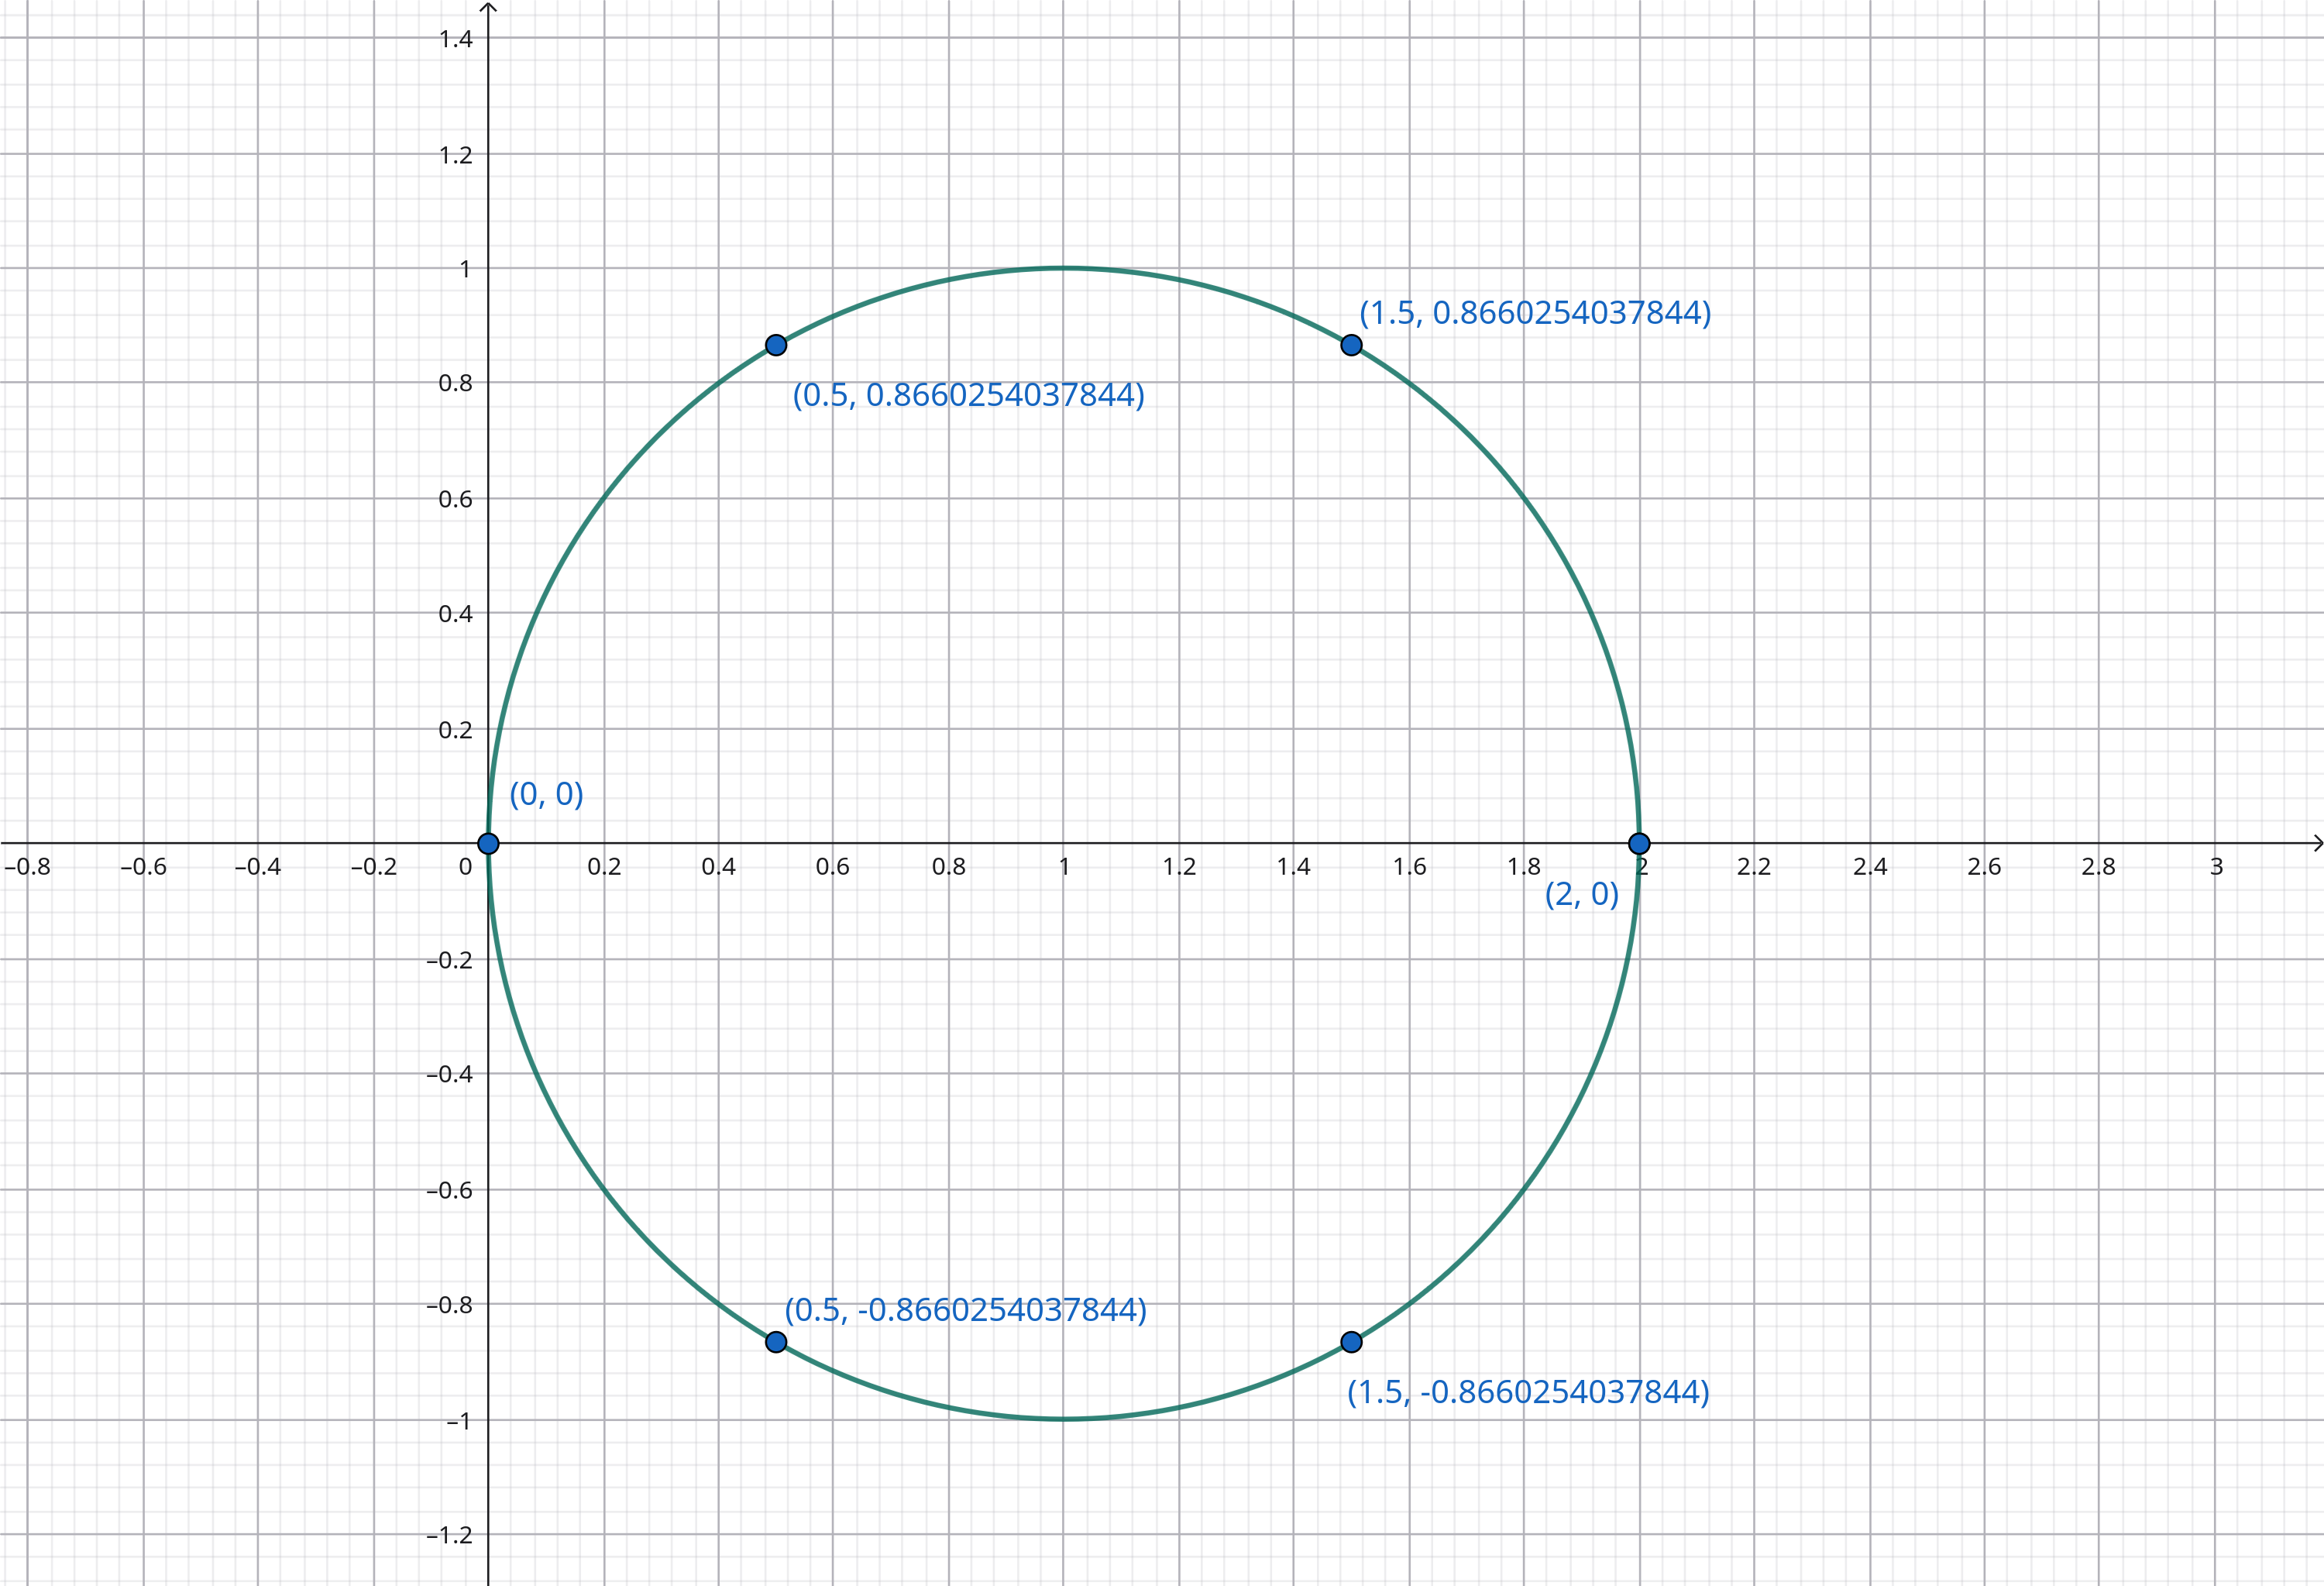
\includegraphics[width=0.8\linewidth]{./geogebra-export2.png}
\end{figure}


% Actividad 3
\section*{Actividad 3}
\textbf{Instrucciones:} Graficar la cardioide $r = 1 + \cos\theta$ utilizando valores de $\theta$ cada $30^\circ$.
\newline

\textbf{Respuesta:} Considerando $(x, y) = (r\cdot\cos\theta, r\cdot\sin\theta)$:

\begin{center}
	\begin{tabular}{| c | c | c | c |}
		\hline
		$\theta$ & $r$ & $(r, \theta)$ & $(x, y)$ \\ \hline
		$0^\circ$ & $1 + \cos0^\circ = 2$ & $(2, 0^\circ)$ & $(2, 0)$ \\
		$30^\circ$ & $1 + \cos30^\circ = 1 + \frac{\sqrt{3}}{2}$ & $(1 +\frac{\sqrt{3}}{2}, 30^\circ)$ & $(\frac{\sqrt{3}}{2} + \frac{3}{4}, \frac{1}{2} + \frac{\sqrt{3}}{4})$ \\
		$60^\circ$ & $1 + \cos60^\circ = \frac{3}{2}$ & $(\frac{3}{2}, 60^\circ)$ & $(\frac{3}{4}, \frac{3\sqrt{3}}{4})$ \\
		$90^\circ$ & $1 + \cos90^\circ = 1$ & $(1, 90^\circ)$ & $(0, 1)$ \\ 
		$120^\circ$ & $1 + \cos120^\circ = \frac{1}{2}$ & $(\frac{1}{2}, 120^\circ)$ & $(-\frac{1}{4}, \frac{\sqrt{3}}{4})$ \\ 
		$150^\circ$ & $1 + \cos150^\circ = 1 - \frac{\sqrt{3}}{2}$ & $(1 - \frac{\sqrt{3}}{2}, 150^\circ)$ & $(-\frac{\sqrt{3}}{2} + \frac{3}{4}, \frac{1}{2} - \frac{\sqrt{3}}{4})$ \\
		$180^\circ$ & $1 + \cos180^\circ = 0$ & $(0, 180^\circ)$ & $(0, 0)$ \\
		$210^\circ$ & $1 + \cos210^\circ = 1 - \frac{\sqrt{3}}{2}$ & $(1 - \frac{\sqrt{3}}{2}, 210^\circ)$ & $(-\frac{\sqrt{3}}{2} + \frac{3}{4}, -\frac{1}{2} + \frac{\sqrt{3}}{4})$ \\
		$240^\circ$ & $1 + \cos240^\circ = \frac{1}{2}$ & $(\frac{1}{2}, 240^\circ)$ & $(-\frac{1}{4}, -\frac{\sqrt{3}}{4})$ \\
		$270^\circ$ & $1 + \cos270^\circ = 1$ & $(1, 270^\circ)$ & $(0, -1)$ \\
		$300^\circ$ & $1 + \cos300^\circ = \frac{3}{2}$ & $(\frac{3}{2}, 300^\circ)$ & $(\frac{3}{4}, -\frac{3\sqrt{3}}{4})$ \\ 
		$330^\circ$ & $1 + \cos330^\circ = 1 + \frac{\sqrt{3}}{2}$ & $(1 + \frac{\sqrt{3}}{2}, 330^\circ)$ & $(\frac{\sqrt{3}}{2} + \frac{3}{4}, -\frac{1}{2} - \frac{\sqrt{3}}{4})$ \\
		$360^\circ$ & $1 + \cos360^\circ = 2$ & $(2, 360^\circ)$ & $(2, 0)$ \\
		\hline
	\end{tabular}
\end{center}

\begin{figure}[htb]
	\centering
	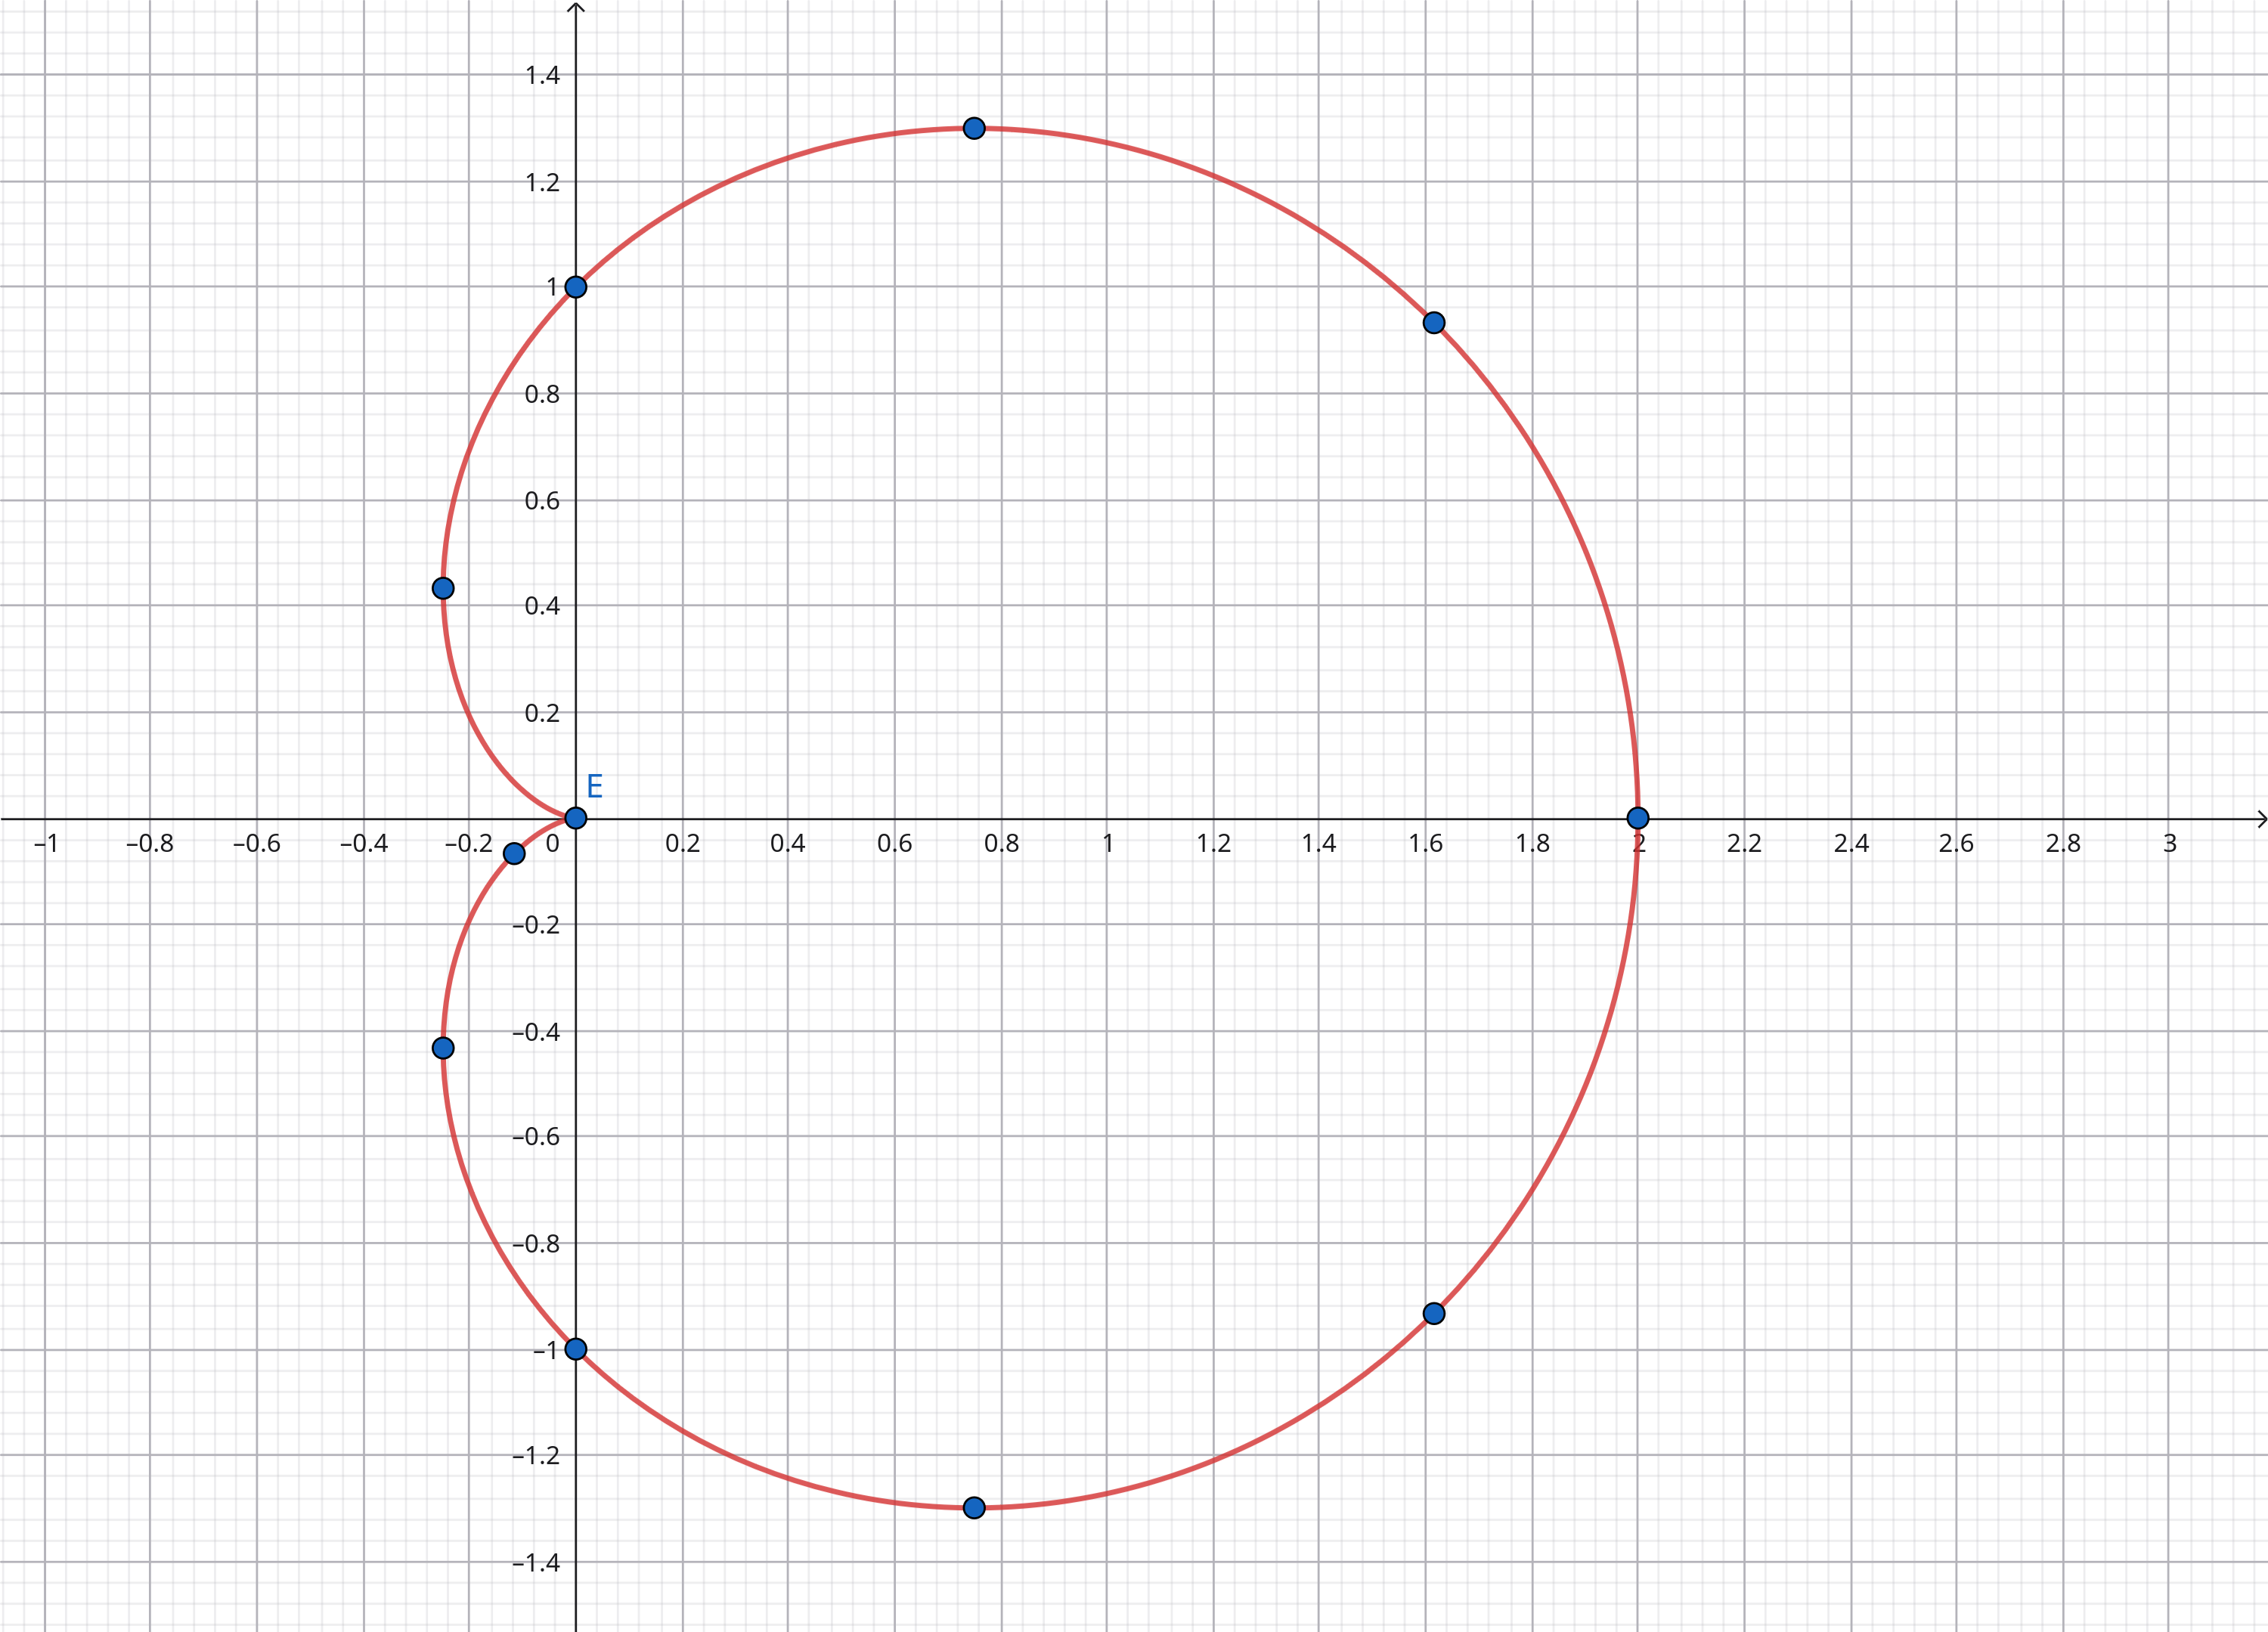
\includegraphics[width=0.8\linewidth]{./geogebra-export3.png}
\end{figure}

\end{document}

